\documentclass{standalone}
\usepackage{tikz, tikz-cd}
\usetikzlibrary{shapes, decorations.markings}
\begin{document}

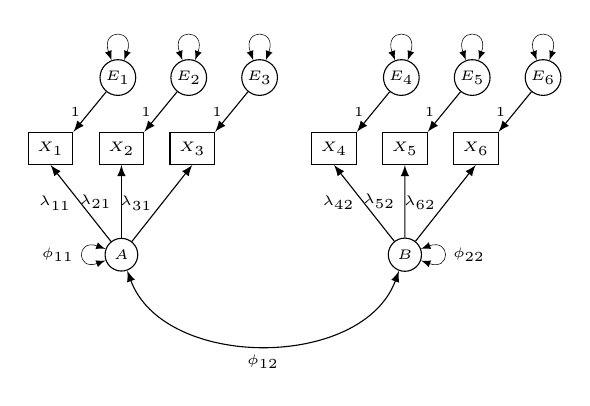
\begin{tikzpicture}[scale=0.9]
\node[draw, circle, inner sep=2] (l1) at (2,2) {\tiny{$A$}};
\node[draw] (o1) at (1,3.5) {\tiny{$X_1$}};
\node[draw] (o2) at (2,3.5) {\tiny{$X_2$}};
\node[draw] (o3) at (3,3.5) {\tiny{$X_3$}};
\node[draw, circle, inner sep=1] (l2) at (1.95,4.5) {\tiny{$E_1$}};
\node[draw, circle, inner sep=1] (l3) at (2.95,4.5) {\tiny{$E_2$}};
\node[draw, circle, inner sep=1] (l4) at (3.95,4.5) {\tiny{$E_3$}};
\node[draw, circle, inner sep=2] (l5) at (6,2) {\tiny{$B$}};
\node[draw] (o4) at (5,3.5) {\tiny{$X_4$}};
\node[draw] (o5) at (6,3.5) {\tiny{$X_5$}};
\node[draw] (o6) at (7,3.5) {\tiny{$X_6$}};
\node[draw, circle, inner sep=1] (l6) at (5.95,4.5) {\tiny{$E_4$}};
\node[draw, circle, inner sep=1] (l7) at (6.95,4.5) {\tiny{$E_5$}};
\node[draw, circle, inner sep=1] (l8) at (7.95,4.5) {\tiny{$E_6$}};
% Arrows
\draw [->, thin, >=latex] (l1)--(o1.south) node[midway, left] {\tiny$\lambda_{11}$};
\draw [->, thin, >=latex] (l1)--(o2.south) node[midway, left] {\tiny$\lambda_{21}$};
\draw [->, thin, >=latex] (l1)--(o3.south) node[midway, left] {\tiny$\lambda_{31}$};
\draw [->, thin, >=latex] (l2)--(o1.north east) node[midway, left] {\tiny$1$};
\draw [->, thin, >=latex] (l3)--(o2.north east) node[midway, left] {\tiny$1$};
\draw [->, thin, >=latex] (l4)--(o3.north east) node[midway, left] {\tiny$1$};
\draw [->, thin, >=latex] (l5)--(o4.south) node[midway, left] {\tiny$\lambda_{42}$};
\draw [->, thin, >=latex] (l5)--(o5.south) node[midway, left] {\tiny$\lambda_{52}$};
\draw [->, thin, >=latex] (l5)--(o6.south) node[midway, left] {\tiny$\lambda_{62}$};
\draw [->, thin, >=latex] (l6)--(o4.north east) node[midway, left] {\tiny$1$};
\draw [->, thin, >=latex] (l7)--(o5.north east) node[midway, left] {\tiny$1$};
\draw [->, thin, >=latex] (l8)--(o6.north east) node[midway, left] {\tiny$1$};
\draw [<->, thin, >=latex] (l1) to [out=290,in=250]  node[midway, below] {\tiny$\phi_{12}$} (l5);
% Residuals:
\draw[<->, very thin, >=latex] (l2) to [out=70,in=110,looseness=7] (l2);
\draw[<->, very thin, >=latex] (l3) to [out=70,in=110,looseness=7] (l3);
\draw[<->, very thin, >=latex] (l4) to [out=70,in=110,looseness=7] (l4);
\draw[<->, very thin, >=latex] (l6) to [out=70,in=110,looseness=7] (l6);
\draw[<->, very thin, >=latex] (l7) to [out=70,in=110,looseness=7] (l7);
\draw[<->, very thin, >=latex] (l8) to [out=70,in=110,looseness=7] (l8);
\draw[<->, very thin, >=latex] (l1) to [out=160,in=200,looseness=7] node[midway, left] {\tiny$\phi_{11}$} (l1);
\draw[<->, very thin, >=latex] (l5) to [out=-20,in=20,looseness=7] node[midway, right] {\tiny$\phi_{22}$}  (l5);
\end{tikzpicture}

\end{document}